% ----------------------------------------------------------------
% AMS-LaTeX Paper ************************************************
% **** -----------------------------------------------------------
\documentclass{amsart}
\usepackage{graphicx}
\usepackage{tikz}
% ----------------------------------------------------------------
\vfuzz2pt % Don't report over-full v-boxes if over-edge is small
\hfuzz2pt % Don't report over-full h-boxes if over-edge is small
% THEOREMS -------------------------------------------------------
\newtheorem{thm}{Theorem}[section]
\newtheorem{cor}[thm]{Corollary}
\newtheorem{lem}[thm]{Lemma}
\newtheorem{prop}[thm]{Proposition}
\theoremstyle{definition}
\newtheorem{defn}[thm]{Definition}
\theoremstyle{remark}
\newtheorem{rem}[thm]{Remark}
\numberwithin{equation}{section}
% MATH -----------------------------------------------------------
\newcommand{\norm}[1]{\left\Vert#1\right\Vert}
\newcommand{\abs}[1]{\left\vert#1\right\vert}
\newcommand{\set}[1]{\left\{#1\right\}}
\newcommand{\Real}{\mathbb R}
\newcommand{\eps}{\varepsilon}
\newcommand{\To}{\longrightarrow}
\newcommand{\BX}{\mathbf{B}(X)}
\newcommand{\A}{\mathcal{A}}
% ----------------------------------------------------------------
\begin{document}

\title{Complex Networks  - Spring 2024\\{\bf Homework 3}}%
\author{Instructor: Jia Liu \\ Solution by: Renan Monteiro Barbosa}%
\date{03/23/2025}

%\dedicatory{}%
%\commby{}%
% ----------------------------------------------------------------

\maketitle
% ----------------------------------------------------------------
\begin{itemize}
\item DUE on  03/23/2025 11:59pm C.T.
\item You can write on the separate work sheet or type your quiz. ( Word or Latex or similar)
\item If you use the handwriting, Solutions must be neat,clear and legible.
\item If you need to scan you quiz, save it as a PDF file. Do not use jpeg, png, jpg etc. Do not submit more than one file.
\item Please check your scanned file before submission. Make sure it is readable, correct order, properly oriented. Make sure it does include all pages.
\item Please name your file as follows: $LastnameInitials-MAP5990quiz1.pdf$.If your name is Alan David Roberts, file name is $RobertsAD-MAP5990quiz1.pdf$.
\item Try to keep the file size less than 4MB.
\item You can resubmit the quiz if you want. Please specify which one is the one to be graded. Otherwise I will grade the most recent version.
\item DO NOT EMAIL me the quiz. All quizzes are submitted via Canvas.
\end{itemize}

\clearpage
\begin{enumerate}

%---------------------------------------------------------------------------------
% ##############################################################################
% Problem 1
% ##############################################################################
\item Consider the adjacency matrix A of a directed network of size $N = 4$ given by \vspace{0.2cm}
\begin{equation*}
{A}  = \left\lbrack\begin{array}{cccc}
0 & 1 & 1 & 0 \\
0 & 0 & 0 & 1 \\
0 & 0 & 0 & 1 \\
0 & 0 & 0 & 0 \\
\end{array}\right\rbrack
\end{equation*}

\vspace{0.2cm}
In the following we will indicate with ${\bf 1}$ the column vector with elements $i_i = 1$ for $i = 1, 2, \cdots, N$ and we will indicate with ${\bf I}$the identity matrix. \vspace{0.2cm}
\begin{enumerate}
\item Draw the network
\item Calculate the eigenvector centrality using its definition.
\item Calculate the Katz centrality.
\item Calculate the PageRank centrality. 
\end{enumerate}
\vspace{1cm}

\textbf{Answers:}

\begin{enumerate}
% #######################
% Problem 1-a
% ####################### 
\item Draw the network. \vspace{0.2cm}

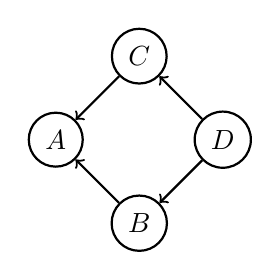
\begin{tikzpicture}[node distance={15mm}, thick, main/.style = {draw, circle}] 
    \node[main] (1) {$A$}; 
    \node[main] (2) [below right of=1] {$B$}; 
    \node[main] (3) [above right of=1] {$C$}; 
    \node[main] (4) [above right of=2] {$D$}; 
    \draw[<-] (1) -- (2); 
    \draw[<-] (1) -- (3);  
    \draw[<-] (2) -- (4); 
    \draw[<-] (3) -- (4); 
\end{tikzpicture}

\vspace{0.2cm}
% #######################
% Problem 1-b
% ####################### 
\item Calculate the eigenvector centrality using its definition. \vspace{0.2cm}

The graph is not strongly connected. Therefore there might be several left eigenvectors associated with 
$\lambda$, and some of their elements might be zero.

If all eigenvalues of a graph's adjacency matrix are zero, and the graph is not strongly connected, then the eigenvector centrality scores for all nodes will likely be zero, as the eigenvector associated with the largest eigenvalue (which eigenvector centrality relies on) will be a zero vector. 

\vspace{0.2cm}
% #######################
% Problem 1-c
% ####################### 
\item Calculate the Katz centrality. \vspace{0.2cm}

Considering alpha = 0.1

Katz centrality of 0: 0.5

Katz centrality of 1: 0.5

Katz centrality of 2: 0.5

Katz centrality of 3: 0.5

% Alpha should be strictly less than the inverse of the largest eigenvalue (lambda) of the adjacency matrix (1/λ). 

There was a typo, I havent heard about a Kate centrality.
\vspace{0.2cm}
% #######################
% Problem 1-d
% ####################### 
\item Calculate the PageRank centrality. \vspace{0.2cm}


% #######################
% Problem 1- Observations
% ####################### 
Observation:
The main difference betwenn Katz and PageRank, is that Katz propagates the full (discounted) weight to all successors oof a node, whereas PageRank (like eigen-vector centrality) splits the weight among all successors.

Katz Centrality: A node is important if it is highly linked or if it is linked from other important nodes.

PageRank: A node is important if it is highly linked or if it is linked from other important nodes that do not link many other pages.

\end{enumerate}
\clearpage

% ##############################################################################
% Problem 2
% ##############################################################################
\item 
Consider the adjacency matrix A of a directed network of size $N = 4$ given by \vspace{0.2cm}
\begin{equation*}
{A}  = \left\lbrack\begin{array}{cccc}
0 & 1 & 1 & 0 \\
1 & 0 & 0 & 1 \\
1 & 0 & 0 & 1 \\
0 & 1 & 1 & 0 \\
\end{array}\right\rbrack
\end{equation*}

\vspace{0.2cm}
In the following we will indicate with ${\bf 1}$ the column vector with elements $i_i = 1$ for $i = 1, 2, \cdots, N$ and we will indicate with ${\bf I}$the identity matrix. \vspace{0.2cm}
\begin{enumerate}
\item Draw the network
\item Calculate the degree centrality.
\end{enumerate}
\vspace{1cm}

\textbf{Answers:}

\begin{enumerate}
% #######################
% Problem 2-a
% ####################### 
\item Draw the network \vspace{0.2cm}

\vspace{0.2cm}
% #######################
% Problem 2-b
% ####################### 
\item Calculate the degree centrality. \vspace{0.2cm}

\vspace{0.2cm}
\end{enumerate}
\clearpage

% ##############################################################################
% Problem 3
% ##############################################################################
\item A network consists of n nodes in a ring, where n is odd. All the nodes have the same closeness centrality. What is it, as a function of n? \vspace{0.2cm}


\begin{figure}[h]
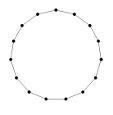
\includegraphics[width=0.2\linewidth]{images/hw3_figure1.PNG}
\end{figure}

\vspace{0.2cm}

\textbf{Answers:}

\clearpage
% ##############################################################################
% Problem 4
% ##############################################################################
\item Study the real-world complex networks on Neuman's website $http://www-personal.umich.edu/~mejn/netdata/$, choose five real-world networks listed in the table and fill the table:

\begin{center}
\begin{tabular}{|c|c|c|c|c|}\hline
Network & directed or not  &node$ \#$	 & edge$ \#$ & community$ \# $ \\ \hline
Karate  & &  &  &   \\ \hline
Dolphin & &  &  &   \\ \hline
Les Miserable& &  &  &   \\ \hline
American College Football & &  &  &   \\ \hline
Power Grid & &  &  &   \\ \hline
\end{tabular}
\end{center}

\vspace{0.2cm}

\textbf{Answers:}

\vspace{5cm}
\clearpage

% ##############################################################################
% Problem 5
% ##############################################################################
\item Choose one network  from the previous question: \vspace{0.2cm}
\begin{enumerate}
\item Use Gephi to plot the network. Make sure to use centrality and communities so that you can show the properties of the network.
\item Use Gephi to find the largest two nodes with the betweenness centrality, degree centrality, and pagerank centrality. Use the table to report  your data.
\end{enumerate}

\vspace{0.5cm}

\textbf{Answers:}

\begin{enumerate}
% #######################
% Problem 5-a
% ####################### 
\item Use Gephi to plot the network. \vspace{0.2cm}

\vspace{0.2cm}
% #######################
% Problem 5-b
% ####################### 
\item Use Gephi to find the largest two nodes \vspace{0.2cm}

\vspace{0.2cm}
\end{enumerate}

\end{enumerate}

\end{document}
% ----------------------------------------------------------------
